\documentclass[a4paper,12pt]{article}

%%% Работа с русским языком
\usepackage{cmap}					% поиск в PDF
\usepackage{mathtext} 				% русские буквы в фомулах
\usepackage[T2A]{fontenc}			% кодировка
\usepackage[utf8]{inputenc}			% кодировка исходного текста
\usepackage[english, russian]{babel}	% локализация и переносы

%%% Дополнительная работа с математикой
\usepackage{amsmath,amsfonts,amssymb,amsthm,mathtools} % AMS
\usepackage{icomma} % "Умная" запятая: $0,2$ --- число, $0, 2$ --- перечисление
%\usepackage{tempora}

%% Номера формул
%\mathtoolsset{showonlyrefs=true} % Показывать номера только у тех формул, на которые есть \eqref{} в тексте.
%\usepackage{leqno} % Немуреация формул слева

%% Свои команды
\DeclareMathOperator{\sgn}{\mathop{sgn}}

%% Перенос знаков в формулах (по Львовскому)
\newcommand*{\hm}[1]{#1\nobreak\discretionary{}
{\hbox{$\mathsurround=0pt #1$}}{}}

%%% Работа с картинками
\usepackage{graphicx}  % Для вставки рисунков
\graphicspath{{Pictures/}} % папки с картинками
\setlength\fboxsep{2pt} % Отступ рамки \fbox{} от рисунка
\setlength\fboxrule{1pt} % Толщина линий рамки \fbox{}
\usepackage{wrapfig} % Обтекание рисунков текстом




%%% Работа с таблицами
\usepackage{array,tabularx,tabulary,booktabs} % Дополнительная работа с таблицами
\usepackage{longtable}  % Длинные таблицы
\usepackage{multirow} % Слияние строк в таблице

%%% Теоремы
\theoremstyle{plain} % Это стиль по умолчанию, его можно не переопределять.
\newtheorem{theorem}{Теорема}[section]
\newtheorem{proposition}[theorem]{Утверждение}

\theoremstyle{definition} % "Определение"
\newtheorem{corollary}{Следствие}[theorem]
\newtheorem{problem}{Задача}[section]

\theoremstyle{remark} % "Примечание"
\newtheorem*{nonum}{Решение}

%%% Программирование
\usepackage{etoolbox} % логические операторы

%%% Страница
\usepackage{extsizes} % Возможность сделать 14-й шрифт
\usepackage{geometry} % Простой способ задавать поля
%Список команд
%----------------------------------------
\newcommand{\grad}
{\mathop{\mathrm{grad}}\nolimits\,} %градиент

\newcommand{\diver}
{\mathop{\mathrm{div}}\nolimits\,} %дивергенция

\newcommand{\rot}
{\ensuremath{\mathrm{rot}}\,}

\newcommand{\Def}[1]
{\underline{\textbf{#1}}} %определение

\newcommand{\RN}[1]
{\MakeUppercase{\romannumeral #1}} %римские цифры

\newcommand {\theornp}[2]
{\textbf{#1.} \textit{ #2} \par} %Написание леммы/теоремы без доказательства

\newcommand{\qrq}
{\ensuremath{\quad \Rightarrow \quad}} %Человеческий знак следствия

\newcommand{\qlrq}
{\ensuremath{\quad \Leftrightarrow \quad}} %Человеческий знак равносильности

\renewcommand{\phi}{\varphi} %Нормальный знак фи

\newcommand{\me}
{\ensuremath{\mathbb{E}}}

\newcommand{\md}
{\ensuremath{\mathbb{D}}}



%\renewcommand{\vec}{\overline}




%----------------------------------------
%Разметка листа
%----------------------------------------
\geometry{top = 3cm}
\geometry{bottom = 2cm}
\geometry{left = 1.5cm}
\geometry{right = 1.5cm}
%----------------------------------------
%\usepackage{fancyhdr} % Колонтитулы
% 	\pagestyle{fancy}
 	%\renewcommand{\headrulewidth}{0pt}  % Толщина линейки, отчеркивающей верхний колонтитул
% 	\lfoot{Нижний левый}
% 	\rfoot{Нижний правый}
% 	\rhead{Верхний правый}
% 	\chead{Верхний в центре}
% 	\lhead{Верхний левый}
%	\cfoot{Нижний в центре} % По умолчанию здесь номер страницы

\usepackage{setspace} % Интерлиньяж
%\onehalfspacing % Интерлиньяж 1.5
%\doublespacing % Интерлиньяж 2
%\singlespacing % Интерлиньяж 1

\usepackage{lastpage} % Узнать, сколько всего страниц в документе.

\usepackage{soul} % Модификаторы начертания

\usepackage{hyperref}
\usepackage[usenames,dvipsnames,svgnames,table,rgb]{xcolor}
\hypersetup{				% Гиперссылки
    unicode=true,           % русские буквы в раздела PDF
    pdftitle={},   % Заголовок
    pdfauthor={Захаров Сергей},      % Автор
    pdfsubject={Отчет по учебной практике},      % Тема
    pdfcreator={Создатель}, % Создатель
    pdfproducer={Производитель}, % Производитель
    pdfkeywords={Учебная практика} {Термокаппилярная неустойчивость}, % Ключевые слова
    colorlinks=true,       	% false: ссылки в рамках; true: цветные ссылки
    linkcolor=red,          % внутренние ссылки
    citecolor=black,        % на библиографию
    filecolor=magenta,      % на файлы
    urlcolor=cyan           % на URL
}

\usepackage{csquotes} % Инструменты для ссылок
\usepackage{cite} % Работа с библиографией
%\usepackage[superscript]{cite} % Ссылки в верхних индексах
%\usepackage[nocompress]{cite} %

\usepackage{float} %force establishe parametr to figure H,h,!

\usepackage{multicol} % Несколько колонок

\usepackage{ mathrsfs }

\usepackage{physics}

\usepackage{mathtools}
\usepackage{mdwtab}

\usepackage{empheq}
\usepackage{floatflt}
\usepackage[most]{tcolorbox}
\usepackage{enumerate}

%\usepackage{floatrow}


\usepackage{tikz}
\usetikzlibrary{fadings}
\usetikzlibrary{shadows.blur}
\usetikzlibrary{shapes}


\usepackage{pgfplots}
\DeclareUnicodeCharacter{2212}{−}
\usepgfplotslibrary{groupplots,dateplot}
\usetikzlibrary{patterns,shapes.arrows}
\pgfplotsset{compat=newest}

\author{Сергей Захаров}

\usepackage{graphicx,xcolor}
\graphicspath{{Pictures/}}
\DeclareGraphicsExtensions{.pdf,.png,.jpg}

\date{\today}

\begin{document}
\thispagestyle{empty}

\begin{center}
	\textit{Федеральное государственное автономное учреждение \\
		высшего профессионального образования}
	\vspace{0.5ex}
	
	\textbf{НАЦИОНАЛЬНЫЙ ИССЛЕДОВАТЕЛЬСКИЙ УНИВЕРСИТЕТ \\ <<ВЫСШАЯ ШКОЛА ЭКОНОМИКИ>>}\\
	\vspace{0.5ex}
	\textbf{Факультет физики}\\
	\vspace{0.5ex}
	\textbf{Бакалавриат}\\
	\vspace{0.5ex}
	\small{\textit{Образовательная программа «Физика» 03.03.02}}
\end{center}
\vspace{7ex}

\begin{center}
	\vspace{2ex}
	{\Large\textbf{О\,Т\,Ч\,Е\,Т}}
	
	{\large\textbf{по учебной практике}} \\
	\vspace{1ex}	
	{по теме:}
	
	\Large{\textbf{\textit{<<Зародышеобразование и рост двумерных пленок йодида никеля
			на поверхности  Ni(110)>>}}}
	

\end{center}
\begin{flushright}
\vspace{30ex}
	\noindent
	Выполнил студент группы БФЗ183\\
	\textit{Захаров Сергей Дмитриевич}\\
\vspace{2ex}
\underline{\hspace{3cm}}\\
  
\end{flushright}
\begin{flushleft}
\vspace{1ex}
	\noindent
	\textbf{Проверил:}\\
	к.ф.-м.н.,
доцент Базовой кафедры\\
квантовых технологий\\
при Институте общей физики\\
им. А.М. Прохорова РАН\\
факультета физики НИУ ВШЭ\\

\textit{Комаров Никита Сергеевич}\\
\vspace{2ex}
\underline{\hspace{3cm}}\\
\vspace{2ex}
\today
\end{flushleft}

\begin{center}
    	\vfill
	Москва \\2021 г.
\end{center}


\newpage

\tableofcontents

\newpage

\section{Актуальность работы}

В последнее время двумерные (2D) галогениды металлов привлекли к себе огромное внимание из-за возможности управления их механическими, электронными, магнитными и топологическими свойствами, в значительной степени пополняя семейство 2D-ван-дер-Ваальсовых (ВДВ) материалов. Особый интерес представляют магнитные двумерные материалы, которые являются перспективными для создания устройств спинтроники \cite{1, 2, 3, 4}.

Следует отметить, что для синтеза 2D ВДВ материалов в настоящее время в основном используется т.н. «скотч-технология» (механическое отщепление тонких слоев от соответствующих объемных кристаллов). Однако отщепленные слои обычно загрязнены внешними примесями и часто имеют большое количество внутренних дефектов, которые приводят к деградации материала. В результате приборы на основе таких слоев имеют плохо воспроизводимые параметры. В этой связи, в качестве технологии создания 2D ВДВ материалов крайне актуальным и перспективным являются сверхвысоковакуумные технологии на основе поверхностных химических реакций и ван-дер-Ваальсовой эпитаксии. В реакции взаимодействия молекулярных галогенов с поверхностью металлов, тонкий слой галогенида формируется как естественный продукт реакции.

%Двумерные материалы являются одним из самых интересных и перспективных направлений современной физики, которое появилось с моментом открытия графена и активно развивается и по сей день. Повышенный интерес к двумерным материалам заключается в том, что при уменьшении симметрии (переходя от трехмерных объектов к двумерным) у одного и того же материала могут кардинально меняться свойства. Одним из интересных для изучения материалов является двумерный йодид никеля \cite{Cool}, работа с которым является темой моей научно-исследовательской работы.

%Одна из задач, которая стоит перед учеными этой области — непосредственно выращивание двумерных материалов. Этот процесс может осуществляться, например, методом скотча, посредством которого и был получен графен. В моей работе предлагается вырастить двумерный NiI$_2$ в том числе посредством поверхностной химической реакцией. Поверхностная химическая реакция позволяет, в отличии от того же метода скотча, производить контролируемый рост пленки материала в заданных условиях.

%Поверхностная химическая реакция, однако, подразумевает, использование в качестве одного из компонентов реакции подложку (т.е. для получения йодида никеля необходимо использовать никелевую подложку). Такой метод доступен не всегда, поэтому актуальным вопросом является изучение другого метода получения двумерных материалов, посредством напыления вещества на поверхность подложки.

\section{Цели и задачи}

Цель   работы: провести сравнительное исследование морфологии и атомной структуры  пленок двумерного йодида никеля (NiI$_{2}$)  на подложке Ni(111), 
полученных как йодированием, в результате прямой адсорбции  молекулярного йода, так и путем напыления из эффузионной ячейки.  

Для достижения поставленной цели решались  задачи:

\begin{enumerate}
	\item Подготовка чистой поверхности Ni(110).
	\item Роста двумерной пленки йодида никеля с использованием поверхностной химической реакции Ni(110) $+$ I$_{2}$.
	\item Охарактеризации поверхности йодида никеля  методами электронной оже-спектроскопии, дифракции медленных электронов, сканирующей туннельной
 микроскопии, термодесорбции.  Установить наличие/отсутствие  полиморфных фазы NiI$_2$ на поверхности Ni(100).
	\item Роста двумерной пленки йодида никеля с использование напылительной ячейки NiI$_2$.
	\item Охарактеризации  поверхности йодида никеля  методами электронной оже-спектроскопии, дифракции медленных электронов, сканирующей туннельной
 микроскопии, термодесорбции.
\end{enumerate}


\section{Экспериментальная установка}

На Рисунке \ref{fig:1_setup} представлена схема сверхвысоковауумной установки, в которой были выполнены все исследования, представленные в данной работе.
Установка состоит из аналитической камеры (1),  СТМ-камеры (3) и шлюзовой камеры (2), использовавшейся для загрузки/выгрузки  образцов  и  зондов (СТМ-игл) сканирующего туннельного микроскопа. Аналитическая камера оснащена оже-спектрометром (5) с анализатором типа <<цилиндрическое зеркало>> (Riber OPC-200), квадрупольным масс-спектрометром (6) (Riber Q-156), сканирующей ионной пушкой (7) (Riber CI-50) и системой напуска газов (8). В СТМ-камере находится вакуумный модуль СТМ (10) (СТМ-GPI300) и дифрактометр медленных электронов (9) с трехсеточным анализатором электронов (Riber OPR 304). Аналитическая камера отделена
от СТМ-камеры  и шлюзовой камеры шиберными затворами (14).  Аналитическая камера и СТМ-камера оснащены системой откачки,
включающей в себя магниторазрядный и титановый сублимационный насосы. Базовое давление в обеих камерах составляет 1$\times$10$^{-10}$ Торр.

 \begin{figure}[t] % Рисунок 1
    \centerline{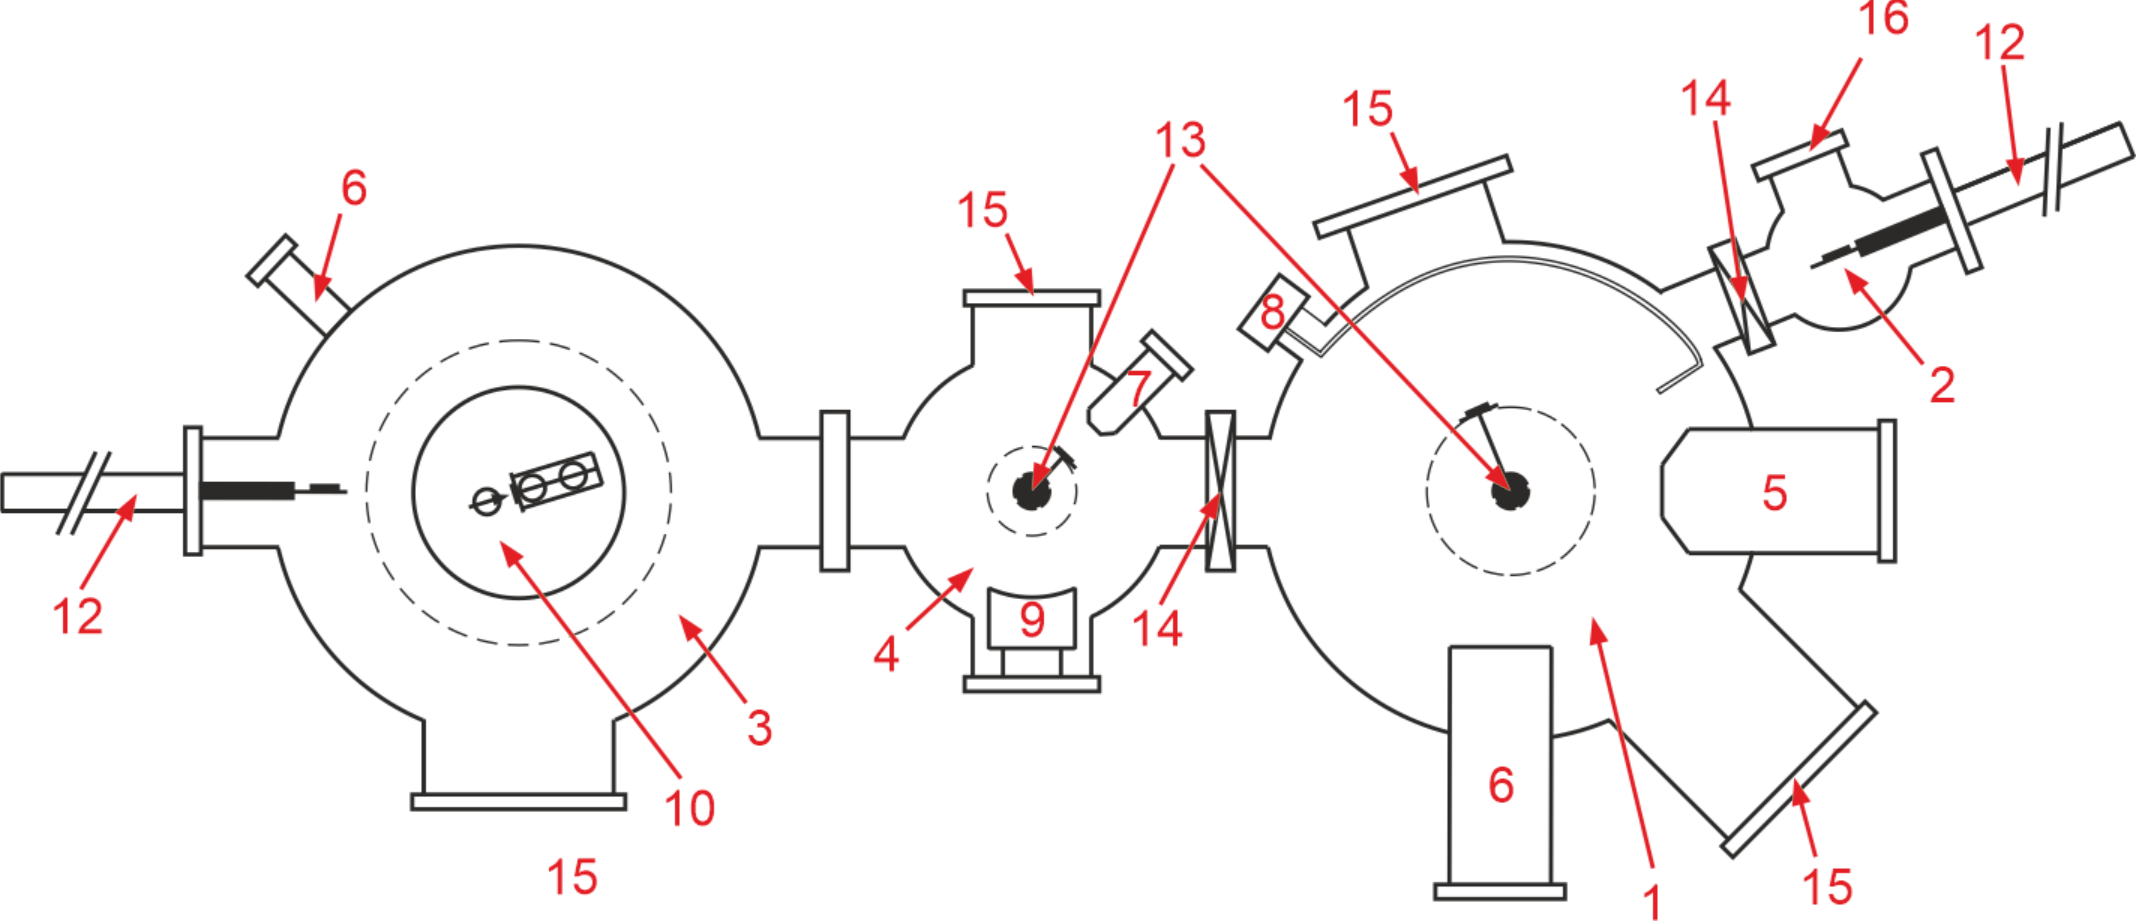
\includegraphics[width=14cm]{Setup.png}}
    \caption{Схемы СВВ-установки. Вид сверху: (1) аналитическая камера, (2) шлюзовая камера, (3) СТМ-камера, (4) ДМЭ-камера, (5) оже-спектрометр, (6) масс-спектрометр, (7) ионная пушка, (8) пьезокерамический натекатель для напуска молекулярного йода, (9) дифрактометр медленных электронов, (10) вакуумный модуль СТМ, (11) электронная пушка, (12) магнитный линейный шток, (13) универсальный манипулятор с пятью степенями свободы, (14) шиберный затвор, (15) смотровое окно, (16) фланец быстрой загрузки, (17) универсальный манипулятор с четырьмя степенями свободы. Картинка взята из работы \cite{Nikita}}
    \label{fig:1_setup}
 \end{figure}

\section{Используемые образцы и методы подготовки чистой поверхности}
 В эксперименте использован монокристаллический образец никеля  Ni(110). Образец изготовлен фирмой Surface Preparation Laboratory (Голландия).
Точность ориентации поверхности относительно заявленной грани была не хуже 0.1$^{\circ}$. Кристалл никеля имеет гранецентрированную кубическую
решетку с периодом $a$ = 3.523 \AA, пространственная группа \emph{Fm3m}.

 Для очистки поверхности Ni(110) применялась серия циклов, состоящих из  последовательного ионного травления ионами аргона в течении 30 минут при
 давлении аргона в камере $2 \cdot 10^{-4}$~Торр и последующего прогрева  при температуре  600$^\circ$C в течении 30 минут.


 \section{Очистка поверхности Ni(110) и последующее йодирование}
 Чистота поверхности контролировалась по оже-спектрам. На рисунке \ref{fig:1_initial} представлен оже-спектр поверхности Ni(110), полученный после внесения образца в
 сверхвысоковакуумную установку. Видно, что помимо оже-пиков никеля (низкоэнергетичный пик 61~эВ, серия пиков около 848~эВ) на рисунке присутствует оже-пик хлора (180 эВ).  В  качестве  критерия химической  чистоты
 поверхности  было  взято  отношение  интенсивностей оже-пиков  характерных  примесей   к  интенсивности  пика  никеля.  Для  чистой поверхности эти отношения
  составляло  порядка 1\%.
  
  % Условия снятия оже; Риски с шагом в 100, сдвинуть ноль (чтобы график с нуля), минорные деления каждые 20, векторную картинку, жирный шрифт, пожирнее сетку сделать

  \begin{figure}[H]
	\centering
	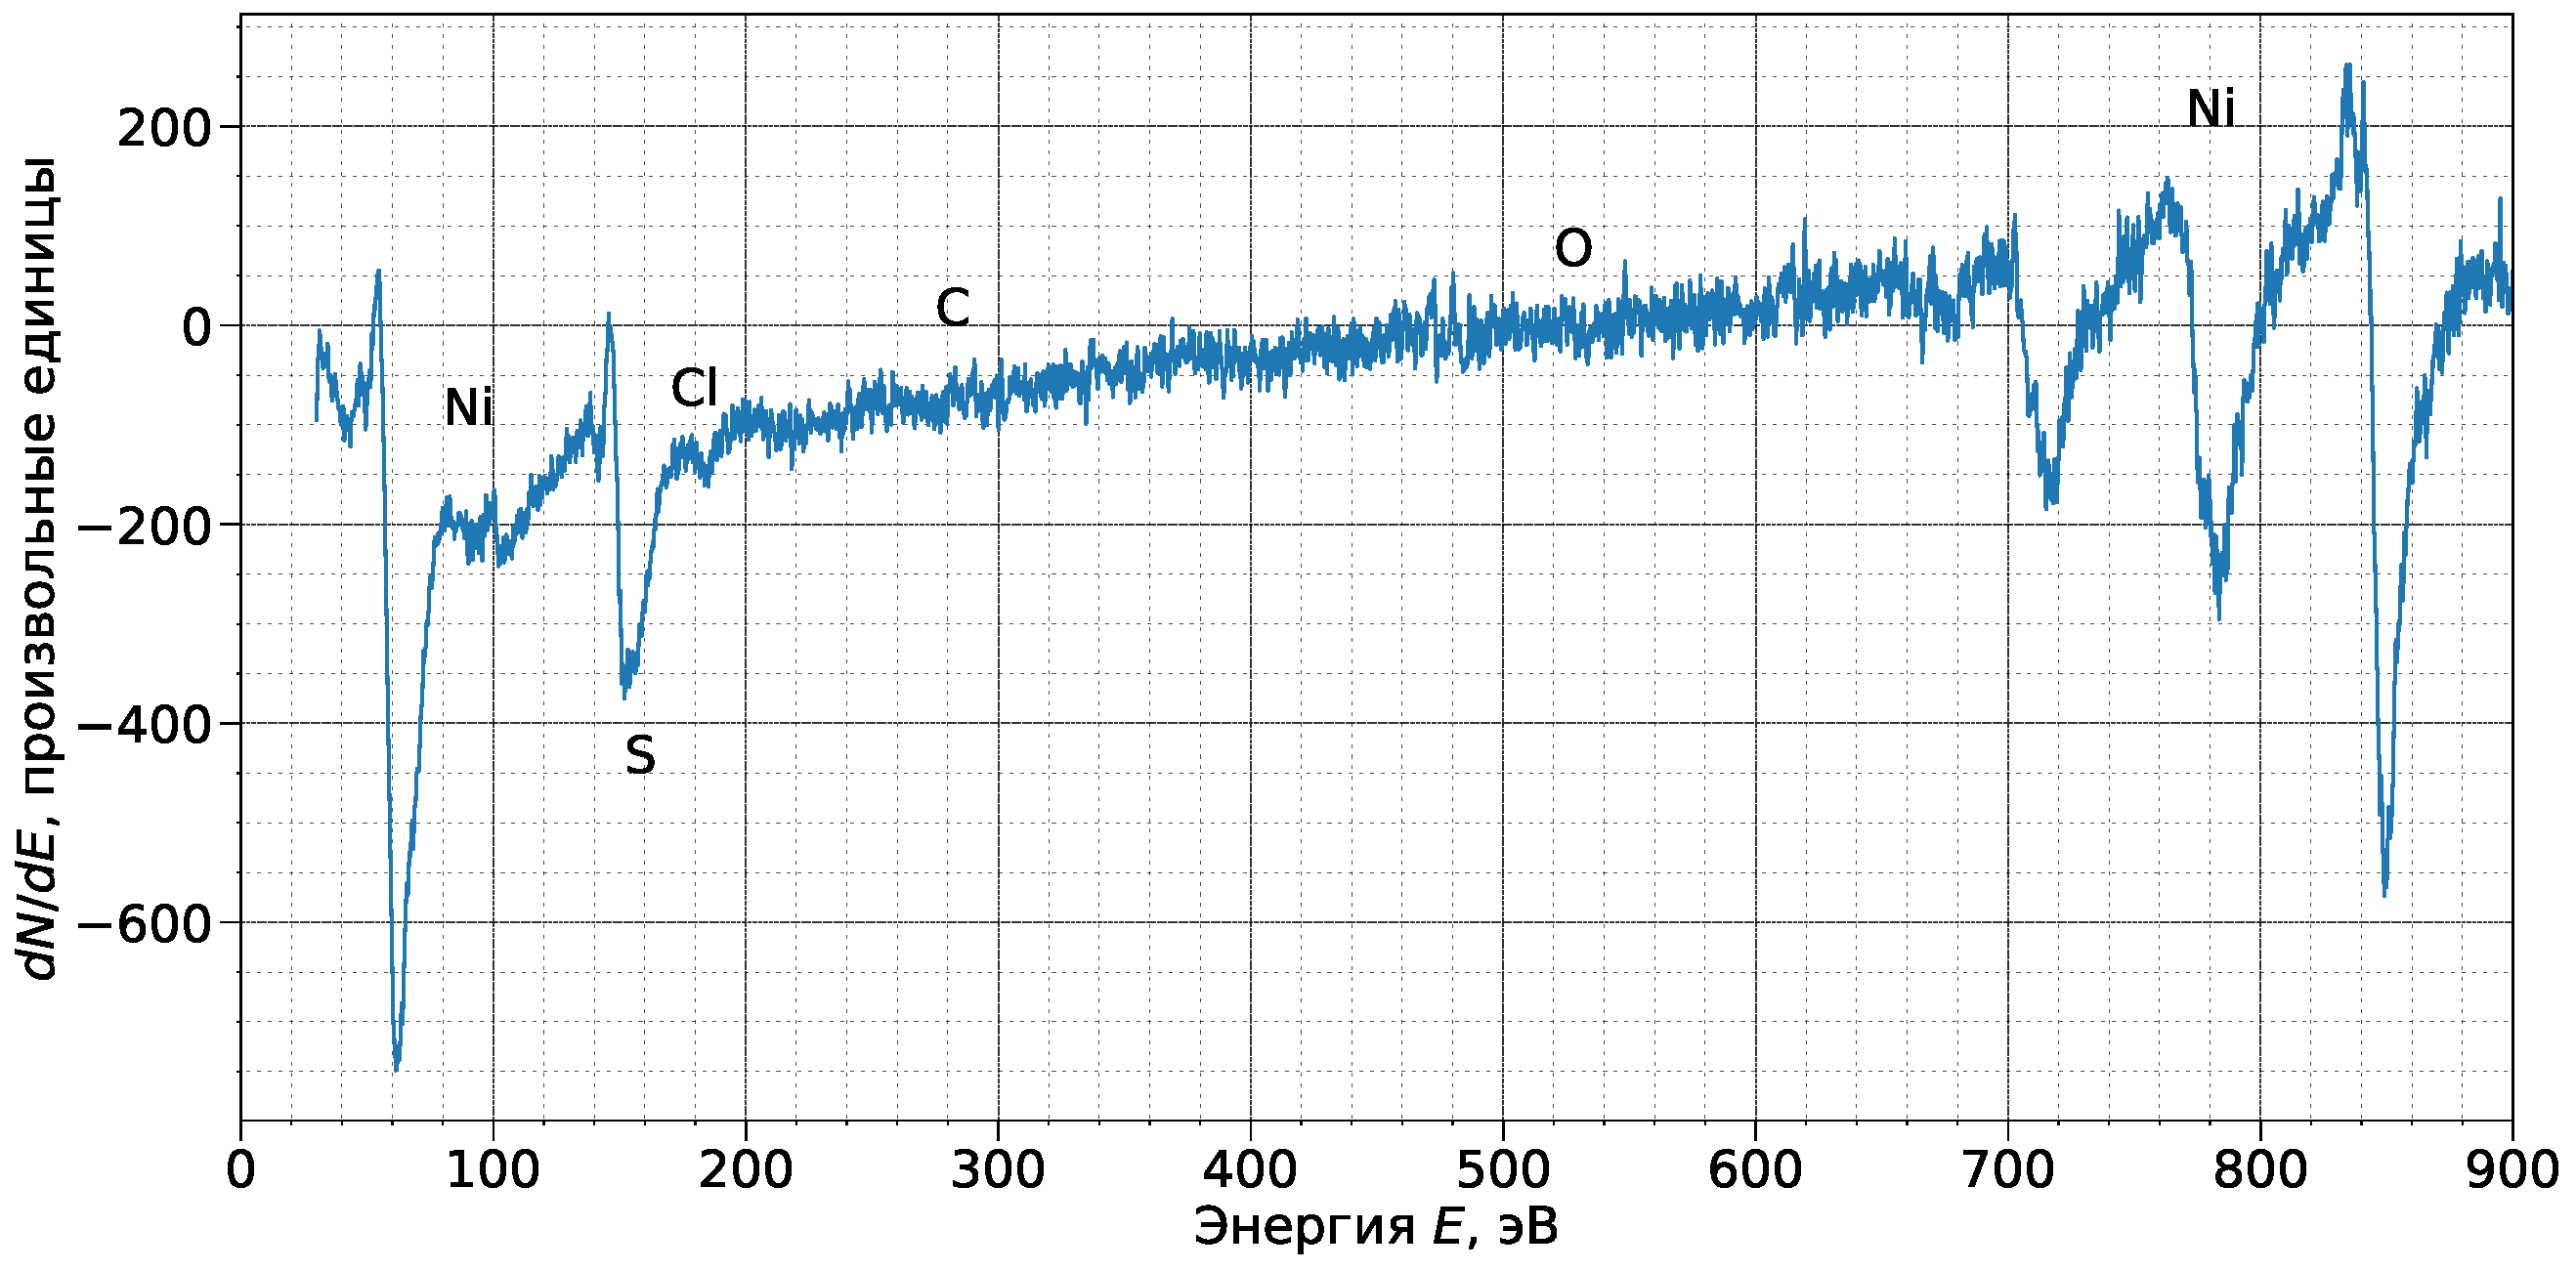
\includegraphics[width=0.9\linewidth]{Initial}
	\caption{Оже-спектр поверхности Ni(110) сразу после внесения образца в сверхвысоковакуумную камеру. $I_e = 2500$~мА, $E_p = 2500$~эВ.}
	\label{fig:1_initial}
\end{figure}

 Поверхность Ni(110) обладает высокой химической  активностью, и поэтому  достаточно быстро становится непригодной для последующей
 адсорбции молекулярного йода.  Для предотвращения загрязнения чистой поверхности Ni(110)  адсорбция молекулярного йода проводилась непосредственно
 после отжига. Данная процедура приводит к формированию пассивирующего слоя йода, который  защищает поверхность от нежелательных загрязнений.
 Напуск йода производился через капилляр на переднюю плоскость образца.  Давлении в камере при напуске йода не опускалась  ниже $4\cdot 10^{-9}$~Торр.
 
 На рисунке \ref{fig:1_final} представлен оже-спектр поверхности Ni(110), полученный после очистки и напуска йода.  Видно, что после очистки поверхности 
 образца оже-пики примесей полностью исчезли. Также на рисунке присутствует   отчетливый оже-пик йода (511 и 520 эВ), что свидетельствует об успешном покрытии поверхности йодом.

\begin{figure}[H]
	\centering
	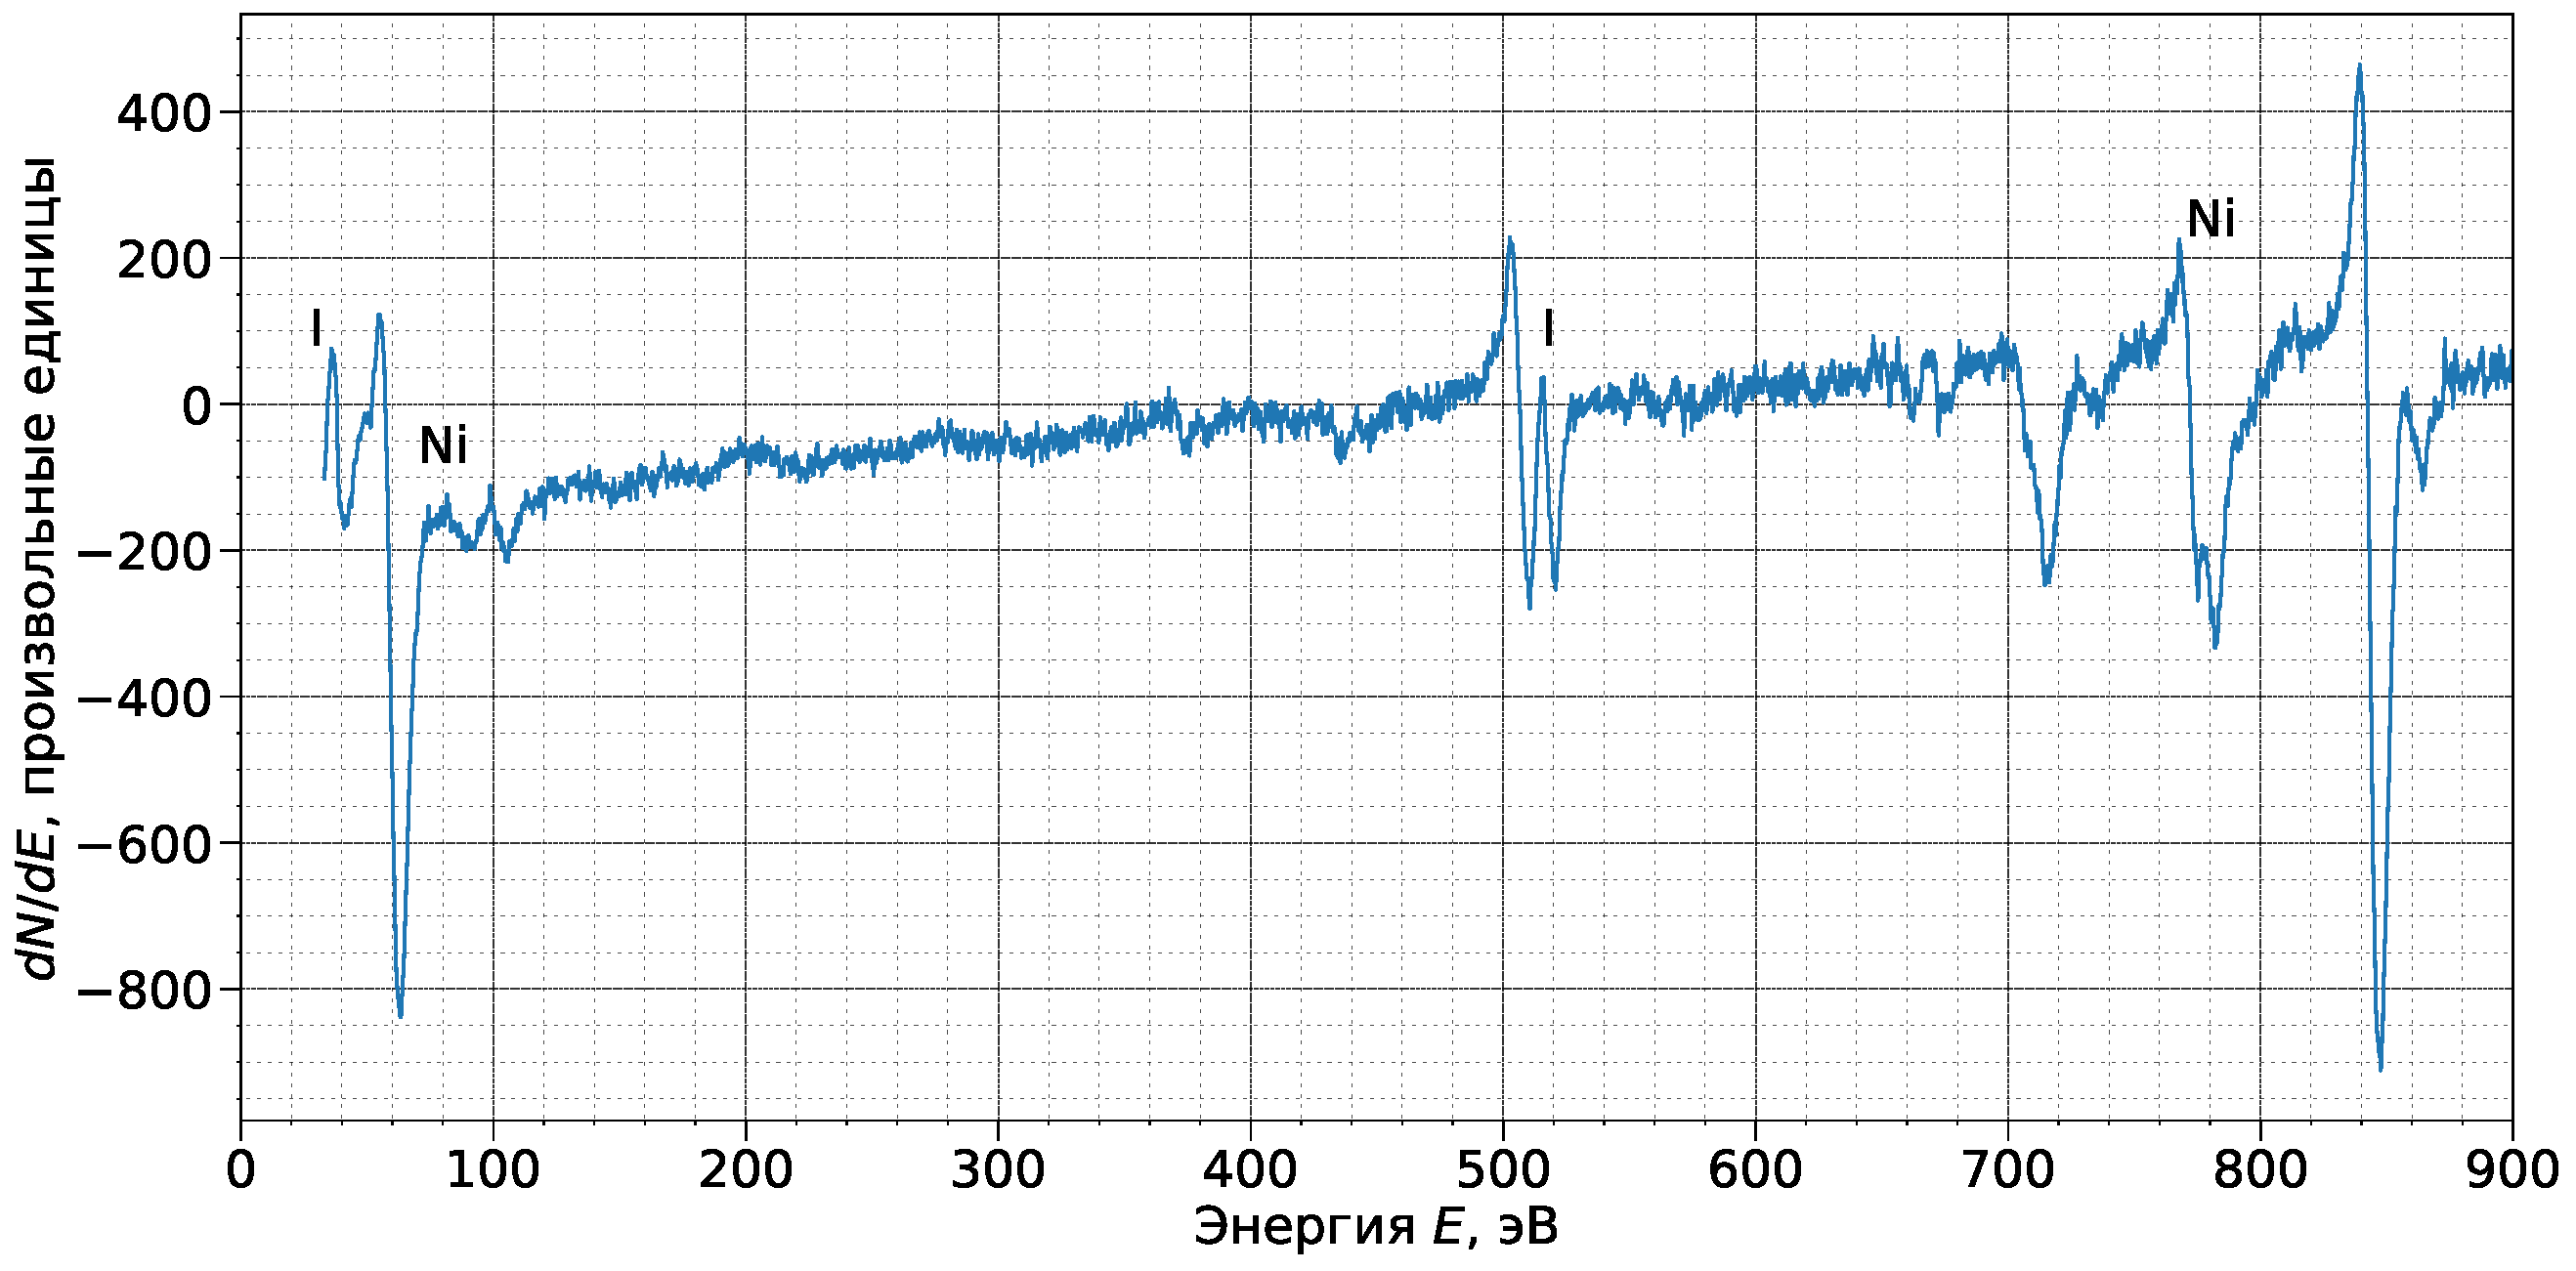
\includegraphics[width=0.9\linewidth]{Final}
	\caption{Оже-спектр поверхности Ni(110) после очистки и напуска йода. $I_e = 2500$~мА,\\$E_p = 2500$~эВ.}
	\label{fig:1_final}
\end{figure}






\begin{thebibliography}{2}
	\bibitem{1} Two-dimensional spintronics for low- power electronics. X. Lin, W. Yang, K. L. Wang, W. Zhao, Nat. Electron. 2, 274 (2019).
    \bibitem{2} Intrinsic Van Der Waals Magnetic Materials from Bulk to the 2D Limit: New Frontiers of Spintronics. H. Li, S. Ruan, Y. J. Zeng,  Adv. Mater. 31, 1900065 (2019).
    \bibitem{3} Prospects and Opportunities of 2D van der Waals Magnetic Systems. Wang, M., Huang, C., Cheung, C., Chen, C., Tan, S. G., Huang, T., Zhao, Y., Zhao, Y., Wu, G., Feng, Y., Wu, H., Chang, C., Annal. Phys. 532, 1900452 (2020).
   \bibitem{4} Magnetism in two-dimensional van der Waals materials. Burch, K.S., Mandrus, D.  Park, J. Nature 563, 47–52 (2018).
	\bibitem{Nikita} Комаров Н.С. Атомные структуры на поверхности монокристаллов никеля при воздействии молекулярного йода
	: дис. к.ф.-м.н.:  01.04.07. - ИОФ РАН, Москва, 2021.
\end{thebibliography}


\end{document} 